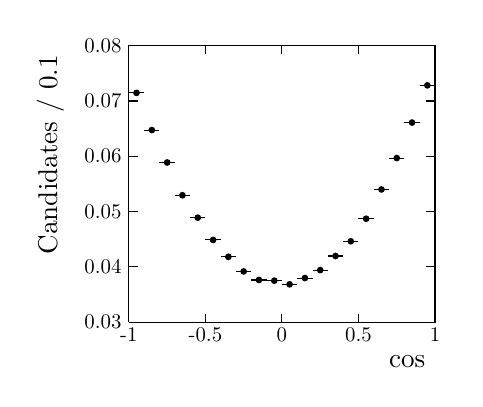
\begin{tikzpicture}
\pgfdeclareplotmark{cross} {
\pgfpathmoveto{\pgfpoint{-0.3\pgfplotmarksize}{\pgfplotmarksize}}
\pgfpathlineto{\pgfpoint{+0.3\pgfplotmarksize}{\pgfplotmarksize}}
\pgfpathlineto{\pgfpoint{+0.3\pgfplotmarksize}{0.3\pgfplotmarksize}}
\pgfpathlineto{\pgfpoint{+1\pgfplotmarksize}{0.3\pgfplotmarksize}}
\pgfpathlineto{\pgfpoint{+1\pgfplotmarksize}{-0.3\pgfplotmarksize}}
\pgfpathlineto{\pgfpoint{+0.3\pgfplotmarksize}{-0.3\pgfplotmarksize}}
\pgfpathlineto{\pgfpoint{+0.3\pgfplotmarksize}{-1.\pgfplotmarksize}}
\pgfpathlineto{\pgfpoint{-0.3\pgfplotmarksize}{-1.\pgfplotmarksize}}
\pgfpathlineto{\pgfpoint{-0.3\pgfplotmarksize}{-0.3\pgfplotmarksize}}
\pgfpathlineto{\pgfpoint{-1.\pgfplotmarksize}{-0.3\pgfplotmarksize}}
\pgfpathlineto{\pgfpoint{-1.\pgfplotmarksize}{0.3\pgfplotmarksize}}
\pgfpathlineto{\pgfpoint{-0.3\pgfplotmarksize}{0.3\pgfplotmarksize}}
\pgfpathclose
\pgfusepathqstroke
}
\pgfdeclareplotmark{cross*} {
\pgfpathmoveto{\pgfpoint{-0.3\pgfplotmarksize}{\pgfplotmarksize}}
\pgfpathlineto{\pgfpoint{+0.3\pgfplotmarksize}{\pgfplotmarksize}}
\pgfpathlineto{\pgfpoint{+0.3\pgfplotmarksize}{0.3\pgfplotmarksize}}
\pgfpathlineto{\pgfpoint{+1\pgfplotmarksize}{0.3\pgfplotmarksize}}
\pgfpathlineto{\pgfpoint{+1\pgfplotmarksize}{-0.3\pgfplotmarksize}}
\pgfpathlineto{\pgfpoint{+0.3\pgfplotmarksize}{-0.3\pgfplotmarksize}}
\pgfpathlineto{\pgfpoint{+0.3\pgfplotmarksize}{-1.\pgfplotmarksize}}
\pgfpathlineto{\pgfpoint{-0.3\pgfplotmarksize}{-1.\pgfplotmarksize}}
\pgfpathlineto{\pgfpoint{-0.3\pgfplotmarksize}{-0.3\pgfplotmarksize}}
\pgfpathlineto{\pgfpoint{-1.\pgfplotmarksize}{-0.3\pgfplotmarksize}}
\pgfpathlineto{\pgfpoint{-1.\pgfplotmarksize}{0.3\pgfplotmarksize}}
\pgfpathlineto{\pgfpoint{-0.3\pgfplotmarksize}{0.3\pgfplotmarksize}}
\pgfpathclose
\pgfusepathqfillstroke
}
\pgfdeclareplotmark{newstar} {
\pgfpathmoveto{\pgfqpoint{0pt}{\pgfplotmarksize}}
\pgfpathlineto{\pgfqpointpolar{44}{0.5\pgfplotmarksize}}
\pgfpathlineto{\pgfqpointpolar{18}{\pgfplotmarksize}}
\pgfpathlineto{\pgfqpointpolar{-20}{0.5\pgfplotmarksize}}
\pgfpathlineto{\pgfqpointpolar{-54}{\pgfplotmarksize}}
\pgfpathlineto{\pgfqpointpolar{-90}{0.5\pgfplotmarksize}}
\pgfpathlineto{\pgfqpointpolar{234}{\pgfplotmarksize}}
\pgfpathlineto{\pgfqpointpolar{198}{0.5\pgfplotmarksize}}
\pgfpathlineto{\pgfqpointpolar{162}{\pgfplotmarksize}}
\pgfpathlineto{\pgfqpointpolar{134}{0.5\pgfplotmarksize}}
\pgfpathclose
\pgfusepathqstroke
}
\pgfdeclareplotmark{newstar*} {
\pgfpathmoveto{\pgfqpoint{0pt}{\pgfplotmarksize}}
\pgfpathlineto{\pgfqpointpolar{44}{0.5\pgfplotmarksize}}
\pgfpathlineto{\pgfqpointpolar{18}{\pgfplotmarksize}}
\pgfpathlineto{\pgfqpointpolar{-20}{0.5\pgfplotmarksize}}
\pgfpathlineto{\pgfqpointpolar{-54}{\pgfplotmarksize}}
\pgfpathlineto{\pgfqpointpolar{-90}{0.5\pgfplotmarksize}}
\pgfpathlineto{\pgfqpointpolar{234}{\pgfplotmarksize}}
\pgfpathlineto{\pgfqpointpolar{198}{0.5\pgfplotmarksize}}
\pgfpathlineto{\pgfqpointpolar{162}{\pgfplotmarksize}}
\pgfpathlineto{\pgfqpointpolar{134}{0.5\pgfplotmarksize}}
\pgfpathclose
\pgfusepathqfillstroke
}
\definecolor{c}{rgb}{1,1,1};
\draw [color=c, fill=c] (0.1,0.0925676) rectangle (4.9,4.53581);
\draw [color=c, fill=c] (0.772,0.803486) rectangle (4.66,4.31365);
\definecolor{c}{rgb}{0,0,0};
\draw [c] (0.772,0.803486) -- (0.772,4.31365) -- (4.66,4.31365) -- (4.66,0.803486) -- (0.772,0.803486);
\draw [c,line width=0.4] (0.8692,3.69605) -- (0.8692,3.71481);
\draw [c,line width=0.4] (0.8692,3.71481) -- (0.8692,3.73358);
\draw [c,line width=0.4] (0.772,3.71481) -- (0.8692,3.71481);
\draw [c,line width=0.4] (0.8692,3.71481) -- (0.9664,3.71481);
\foreach \P in {(0.8692,3.71481)}{\draw[mark options={color=c,fill=c},mark size=1.201201pt,mark=*,mark size=1pt] plot coordinates {\P};}
\draw [c,line width=0.4] (1.0636,3.22469) -- (1.0636,3.24256);
\draw [c,line width=0.4] (1.0636,3.24256) -- (1.0636,3.26042);
\draw [c,line width=0.4] (0.9664,3.24256) -- (1.0636,3.24256);
\draw [c,line width=0.4] (1.0636,3.24256) -- (1.1608,3.24256);
\foreach \P in {(1.0636,3.24256)}{\draw[mark options={color=c,fill=c},mark size=1.201201pt,mark=*,mark size=1pt] plot coordinates {\P};}
\draw [c,line width=0.4] (1.258,2.81357) -- (1.258,2.83061);
\draw [c,line width=0.4] (1.258,2.83061) -- (1.258,2.84764);
\draw [c,line width=0.4] (1.1608,2.83061) -- (1.258,2.83061);
\draw [c,line width=0.4] (1.258,2.83061) -- (1.3552,2.83061);
\foreach \P in {(1.258,2.83061)}{\draw[mark options={color=c,fill=c},mark size=1.201201pt,mark=*,mark size=1pt] plot coordinates {\P};}
\draw [c,line width=0.4] (1.4524,2.39836) -- (1.4524,2.41451);
\draw [c,line width=0.4] (1.4524,2.41451) -- (1.4524,2.43066);
\draw [c,line width=0.4] (1.3552,2.41451) -- (1.4524,2.41451);
\draw [c,line width=0.4] (1.4524,2.41451) -- (1.5496,2.41451);
\foreach \P in {(1.4524,2.41451)}{\draw[mark options={color=c,fill=c},mark size=1.201201pt,mark=*,mark size=1pt] plot coordinates {\P};}
\draw [c,line width=0.4] (1.6468,2.11424) -- (1.6468,2.12977);
\draw [c,line width=0.4] (1.6468,2.12977) -- (1.6468,2.14529);
\draw [c,line width=0.4] (1.5496,2.12977) -- (1.6468,2.12977);
\draw [c,line width=0.4] (1.6468,2.12977) -- (1.744,2.12977);
\foreach \P in {(1.6468,2.12977)}{\draw[mark options={color=c,fill=c},mark size=1.201201pt,mark=*,mark size=1pt] plot coordinates {\P};}
\draw [c,line width=0.4] (1.8412,1.83212) -- (1.8412,1.84699);
\draw [c,line width=0.4] (1.8412,1.84699) -- (1.8412,1.86186);
\draw [c,line width=0.4] (1.744,1.84699) -- (1.8412,1.84699);
\draw [c,line width=0.4] (1.8412,1.84699) -- (1.9384,1.84699);
\foreach \P in {(1.8412,1.84699)}{\draw[mark options={color=c,fill=c},mark size=1.201201pt,mark=*,mark size=1pt] plot coordinates {\P};}
\draw [c,line width=0.4] (2.0356,1.61844) -- (2.0356,1.6328);
\draw [c,line width=0.4] (2.0356,1.6328) -- (2.0356,1.64715);
\draw [c,line width=0.4] (1.9384,1.6328) -- (2.0356,1.6328);
\draw [c,line width=0.4] (2.0356,1.6328) -- (2.1328,1.6328);
\foreach \P in {(2.0356,1.6328)}{\draw[mark options={color=c,fill=c},mark size=1.201201pt,mark=*,mark size=1pt] plot coordinates {\P};}
\draw [c,line width=0.4] (2.23,1.43343) -- (2.23,1.44732);
\draw [c,line width=0.4] (2.23,1.44732) -- (2.23,1.46121);
\draw [c,line width=0.4] (2.1328,1.44732) -- (2.23,1.44732);
\draw [c,line width=0.4] (2.23,1.44732) -- (2.3272,1.44732);
\foreach \P in {(2.23,1.44732)}{\draw[mark options={color=c,fill=c},mark size=1.201201pt,mark=*,mark size=1pt] plot coordinates {\P};}
\draw [c,line width=0.4] (2.4244,1.32496) -- (2.4244,1.33858);
\draw [c,line width=0.4] (2.4244,1.33858) -- (2.4244,1.35219);
\draw [c,line width=0.4] (2.3272,1.33858) -- (2.4244,1.33858);
\draw [c,line width=0.4] (2.4244,1.33858) -- (2.5216,1.33858);
\foreach \P in {(2.4244,1.33858)}{\draw[mark options={color=c,fill=c},mark size=1.201201pt,mark=*,mark size=1pt] plot coordinates {\P};}
\draw [c,line width=0.4] (2.6188,1.31614) -- (2.6188,1.32973);
\draw [c,line width=0.4] (2.6188,1.32973) -- (2.6188,1.34332);
\draw [c,line width=0.4] (2.5216,1.32973) -- (2.6188,1.32973);
\draw [c,line width=0.4] (2.6188,1.32973) -- (2.716,1.32973);
\foreach \P in {(2.6188,1.32973)}{\draw[mark options={color=c,fill=c},mark size=1.201201pt,mark=*,mark size=1pt] plot coordinates {\P};}
\draw [c,line width=0.4] (2.8132,1.27006) -- (2.8132,1.28354);
\draw [c,line width=0.4] (2.8132,1.28354) -- (2.8132,1.29701);
\draw [c,line width=0.4] (2.716,1.28354) -- (2.8132,1.28354);
\draw [c,line width=0.4] (2.8132,1.28354) -- (2.9104,1.28354);
\foreach \P in {(2.8132,1.28354)}{\draw[mark options={color=c,fill=c},mark size=1.201201pt,mark=*,mark size=1pt] plot coordinates {\P};}
\draw [c,line width=0.4] (3.0076,1.34926) -- (3.0076,1.36294);
\draw [c,line width=0.4] (3.0076,1.36294) -- (3.0076,1.37662);
\draw [c,line width=0.4] (2.9104,1.36294) -- (3.0076,1.36294);
\draw [c,line width=0.4] (3.0076,1.36294) -- (3.1048,1.36294);
\foreach \P in {(3.0076,1.36294)}{\draw[mark options={color=c,fill=c},mark size=1.201201pt,mark=*,mark size=1pt] plot coordinates {\P};}
\draw [c,line width=0.4] (3.202,1.45016) -- (3.202,1.4641);
\draw [c,line width=0.4] (3.202,1.4641) -- (3.202,1.47804);
\draw [c,line width=0.4] (3.1048,1.4641) -- (3.202,1.4641);
\draw [c,line width=0.4] (3.202,1.4641) -- (3.2992,1.4641);
\foreach \P in {(3.202,1.4641)}{\draw[mark options={color=c,fill=c},mark size=1.201201pt,mark=*,mark size=1pt] plot coordinates {\P};}
\draw [c,line width=0.4] (3.3964,1.62867) -- (3.3964,1.64305);
\draw [c,line width=0.4] (3.3964,1.64305) -- (3.3964,1.65743);
\draw [c,line width=0.4] (3.2992,1.64305) -- (3.3964,1.64305);
\draw [c,line width=0.4] (3.3964,1.64305) -- (3.4936,1.64305);
\foreach \P in {(3.3964,1.64305)}{\draw[mark options={color=c,fill=c},mark size=1.201201pt,mark=*,mark size=1pt] plot coordinates {\P};}
\draw [c,line width=0.4] (3.5908,1.81538) -- (3.5908,1.83021);
\draw [c,line width=0.4] (3.5908,1.83021) -- (3.5908,1.84504);
\draw [c,line width=0.4] (3.4936,1.83021) -- (3.5908,1.83021);
\draw [c,line width=0.4] (3.5908,1.83021) -- (3.688,1.83021);
\foreach \P in {(3.5908,1.83021)}{\draw[mark options={color=c,fill=c},mark size=1.201201pt,mark=*,mark size=1pt] plot coordinates {\P};}
\draw [c,line width=0.4] (3.7852,2.10093) -- (3.7852,2.11643);
\draw [c,line width=0.4] (3.7852,2.11643) -- (3.7852,2.13192);
\draw [c,line width=0.4] (3.688,2.11643) -- (3.7852,2.11643);
\draw [c,line width=0.4] (3.7852,2.11643) -- (3.8824,2.11643);
\foreach \P in {(3.7852,2.11643)}{\draw[mark options={color=c,fill=c},mark size=1.201201pt,mark=*,mark size=1pt] plot coordinates {\P};}
\draw [c,line width=0.4] (3.9796,2.47205) -- (3.9796,2.48836);
\draw [c,line width=0.4] (3.9796,2.48836) -- (3.9796,2.50468);
\draw [c,line width=0.4] (3.8824,2.48836) -- (3.9796,2.48836);
\draw [c,line width=0.4] (3.9796,2.48836) -- (4.0768,2.48836);
\foreach \P in {(3.9796,2.48836)}{\draw[mark options={color=c,fill=c},mark size=1.201201pt,mark=*,mark size=1pt] plot coordinates {\P};}
\draw [c,line width=0.4] (4.174,2.86962) -- (4.174,2.88677);
\draw [c,line width=0.4] (4.174,2.88677) -- (4.174,2.90392);
\draw [c,line width=0.4] (4.0768,2.88677) -- (4.174,2.88677);
\draw [c,line width=0.4] (4.174,2.88677) -- (4.2712,2.88677);
\foreach \P in {(4.174,2.88677)}{\draw[mark options={color=c,fill=c},mark size=1.201201pt,mark=*,mark size=1pt] plot coordinates {\P};}
\draw [c,line width=0.4] (4.3684,3.3197) -- (4.3684,3.33775);
\draw [c,line width=0.4] (4.3684,3.33775) -- (4.3684,3.3558);
\draw [c,line width=0.4] (4.2712,3.33775) -- (4.3684,3.33775);
\draw [c,line width=0.4] (4.3684,3.33775) -- (4.4656,3.33775);
\foreach \P in {(4.3684,3.33775)}{\draw[mark options={color=c,fill=c},mark size=1.201201pt,mark=*,mark size=1pt] plot coordinates {\P};}
\draw [c,line width=0.4] (4.5628,3.79128) -- (4.5628,3.81022);
\draw [c,line width=0.4] (4.5628,3.81022) -- (4.5628,3.82917);
\draw [c,line width=0.4] (4.4656,3.81022) -- (4.5628,3.81022);
\draw [c,line width=0.4] (4.5628,3.81022) -- (4.66,3.81022);
\foreach \P in {(4.5628,3.81022)}{\draw[mark options={color=c,fill=c},mark size=1.201201pt,mark=*,mark size=1pt] plot coordinates {\P};}
\draw [c,line width=0.4] (0.772,0.803486) -- (4.66,0.803486);
\draw [anchor= east] (4.66,0.305843) node[scale=0.979298, rotate=0]{$\cos\thetaK$};
\draw [c,line width=0.4] (0.772,0.911457) -- (0.772,0.803486);
\draw [c,line width=0.4] (1.744,0.911457) -- (1.744,0.803486);
\draw [c,line width=0.4] (2.716,0.911457) -- (2.716,0.803486);
\draw [c,line width=0.4] (3.688,0.911457) -- (3.688,0.803486);
\draw [c,line width=0.4] (4.66,0.911457) -- (4.66,0.803486);
\draw [anchor=base] (0.772,0.563551) node[scale=0.753306, rotate=0]{-1};
\draw [anchor=base] (1.744,0.563551) node[scale=0.753306, rotate=0]{-0.5};
\draw [anchor=base] (2.716,0.563551) node[scale=0.753306, rotate=0]{0};
\draw [anchor=base] (3.688,0.563551) node[scale=0.753306, rotate=0]{0.5};
\draw [anchor=base] (4.66,0.563551) node[scale=0.753306, rotate=0]{1};
\draw [c,line width=0.4] (0.772,4.31365) -- (4.66,4.31365);
\draw [c,line width=0.4] (0.772,4.20568) -- (0.772,4.31365);
\draw [c,line width=0.4] (1.744,4.20568) -- (1.744,4.31365);
\draw [c,line width=0.4] (2.716,4.20568) -- (2.716,4.31365);
\draw [c,line width=0.4] (3.688,4.20568) -- (3.688,4.31365);
\draw [c,line width=0.4] (4.66,4.20568) -- (4.66,4.31365);
\draw [c,line width=0.4] (0.772,0.803486) -- (0.772,4.31365);
\draw [anchor= east] (-0.2264,4.31365) node[scale=0.979298, rotate=90]{Candidates / 0.1};
\draw [c,line width=0.4] (0.88576,0.803486) -- (0.772,0.803486);
\draw [c,line width=0.4] (0.88576,1.50552) -- (0.772,1.50552);
\draw [c,line width=0.4] (0.88576,2.20755) -- (0.772,2.20755);
\draw [c,line width=0.4] (0.88576,2.90958) -- (0.772,2.90958);
\draw [c,line width=0.4] (0.88576,3.61162) -- (0.772,3.61162);
\draw [c,line width=0.4] (0.88576,4.31365) -- (0.772,4.31365);
\draw [anchor= east] (0.772,0.803486) node[scale=0.753306, rotate=0]{0.03};
\draw [anchor= east] (0.772,1.50552) node[scale=0.753306, rotate=0]{0.04};
\draw [anchor= east] (0.772,2.20755) node[scale=0.753306, rotate=0]{0.05};
\draw [anchor= east] (0.772,2.90958) node[scale=0.753306, rotate=0]{0.06};
\draw [anchor= east] (0.772,3.61162) node[scale=0.753306, rotate=0]{0.07};
\draw [anchor= east] (0.772,4.31365) node[scale=0.753306, rotate=0]{0.08};
\draw [c,line width=0.4] (4.66,0.803486) -- (4.66,4.31365);
\draw [c,line width=0.4] (4.54624,0.803486) -- (4.66,0.803486);
\draw [c,line width=0.4] (4.54624,1.50552) -- (4.66,1.50552);
\draw [c,line width=0.4] (4.54624,2.20755) -- (4.66,2.20755);
\draw [c,line width=0.4] (4.54624,2.90958) -- (4.66,2.90958);
\draw [c,line width=0.4] (4.54624,3.61162) -- (4.66,3.61162);
\draw [c,line width=0.4] (4.54624,4.31365) -- (4.66,4.31365);
\end{tikzpicture}
